\section{\texorpdfstring{Sudo-sudomesta, Prostor cyklu grafu}{Sudo-sudomesta, Prostor cyklu grafu}}
\vspace{5mm}
\large

\begin{theorem}[Sudo-sudomesta]
	Necht $A_1, ... , A_k$ jsou ruzne $ \subseteq [n]$, $ |A_i| = 0 \mod2 \ \forall i, |A_i \cap A_j| \equiv 0 \mod2, i \ne j \Rightarrow k \leq n$
\end{theorem}
\begin{proof}
	Udelame bijekci mnozina $\to$ charakteristicky vektor. Pak lin kombinace je taky sudo-sudomesto. Dal
	\[ \langle A_i, A_j \rangle = \sum_{x \in X} (A_i)_x (A_j)_x = \sum_{x \in A_i \cap A_j} 1 = |A_i \cap A_j| \mod2 \]
	\[ \langle A_i, A_i \rangle = |A_i| \]
	Pak $ \langle A_i, A_j \rangle = 0 \mod2 $. Vezmeme $ m = \sum b_iA_i $, tak
	\[ \langle A_i, m \rangle = \langle A_i, \sum b_iA_i \rangle = \sum b_i \langle A_i, A_j \rangle = 0 \]
	\[ \langle m,m \rangle = \langle \sum b_iA_i, m \rangle = \sum b_i \langle A_i, m \rangle = 0 \]

	Z toho maximalni (vzhledem k inkluzi) system tvorici sudo-sudomesto je nutne podpostor.
	\[ \forall x \in M \forall y \in M \langle x, y \rangle = 0 \Rightarrow \forall x \in M: x \in M^{\perp} \Rightarrow M \subseteq M^{\perp} \]
	\[ \langle M \rangle \subseteq M^{\perp} \Rightarrow dim M \leq dim M^{\perp} = n - dim M \Rightarrow dim \langle M \rangle \leq \lfloor n/2 \rfloor \Rightarrow dim M \leq \lfloor n/2 \rfloor \]

	Odhad je tesny: spojime body do 2jic tvorici rozdklad X. Pak mnoziny budou vsechny mozne podmnoziny obsahujici 2ce. Je jich $ 2^{\lfloor n/2 \rfloor} $
\end{proof}


\begin{definition}
Uvazme bijekci mezi napnutym podgrafem H a jeho charakteristickym vektorem. Mnozina vsech napnutych podgrafu $\nu_G$ tvori V.P. nad $\Z_2$, scitani vektoru odpovida symmetricke diferenci mnoziny hran.
\end{definition}
\begin{definition}
	Mnozina napnutych podgrafu je Eulerovska pokud $\forall u \in V, deg(u) = 0 \mod2$. Znacime $\xi_G$. Pak $\beta_G$ je mnozina elementarnich rezu, t.j. $B_A = (V, \{xy: x \in A, y\in V\setminus A, xy\in E\}), A \subseteq V$.
\end{definition}

\begin{theorem}[Eulerovske grafu]
	$\xi_G, \beta_G$ jsou V.P. podprostory $\nu_G$. Plati $\xi_G^{\perp} = \beta_G \land \beta_G^{\perp} = \xi_G$. Pokud navic je graf souvisly, $dim(\beta_G) = |V| - 1 \land dim(\xi_G) = |E| - |V| + 1$.
\end{theorem}
\begin{proof}
	1) Nasobeni skalarem je automaticky splneno, protoze teleso je $\Z_2$.

	2) $H_1 + H_2 = (V_1, E(H_1) \div E(H_2))$. Taky patri do V.P.

	3) Ukazeme $\forall H_1, H_2 \in \xi_G: H_1 + H_2 \in \xi_G$. Zvolme vrchol u, necht $deg_{H_1} u = 2k, deg_{H_2} u = 2l$, taky h je pocet spolecnych hran obou podgrafu.
	\[ deg_{H_1 + H_2} u = 2k - h + 2l - h = 2k + 2l - 2h \equiv 0 \mod2 \]
	Soucet 2 Eulerovskych grafu je Eulerovsky graf.

	4) Ukazeme $\forall A,Z \subseteq V(G): B_A + B_Z \in \beta_G$.

	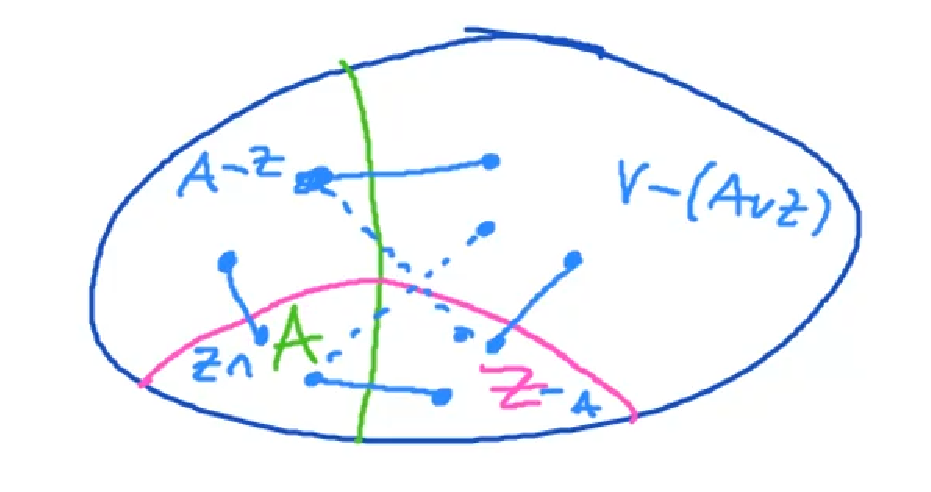
\includegraphics[scale=0.4]{el_rezy.eps}

	Z obrazku prezijou pouze hrany vedouci z $A - Z$ do $V - (Z\cup A)$, hrany z $A - Z$ do $Z \cup A$, hrany $(Z \cap A)$ do $Z - A$ a hrany ze $Z - A$ do $V - (Z\cup A)$. Ostatni byly ve 2 rezich. Zustane rez $B_{A \div Z}, A \div Z = (A - Z) \cup (Z - A)$.
	\[ B_A + B_Z = B_{A \div Z}\]

	Tvrdime ze $B_G = \langle B_{\{u\}}, u \in V \rangle$. Prostor el. rezu je generovany hvezdami. Protoze
	\[ B_A = \sum_{u \in A} B_{\{u\}} \]
	Hrany uvnitr A se smazou sym. diferenci, hrany vedouci ven z A, ktere nejsou spolecne zustanou.

	5) G souvisly $\Rightarrow dim B_G = |V| - 1$. Nahledneme ze secteni vsech hvezd dava $\emptyset$ graf. Neboli kazda hrana patri je 2 hvezdam.

	Zafixujeme vrchol u, secteme hvezdy krome u. $ \sum_{a \ne u} B_{\{a\}} = \emptyset - B_{\{u\}} = B_{\{u\}} \ne \emptyset $
	Pokud vezmeme vsechny krome 1 hvezdy, tak jsou LN a generuji vsechny rezy. Z toho $\Rightarrow dim B_G = |V| - 1$.

	Pozorovani:
	\[ \forall H \subseteq V: H \in \xi_G \iff \langle H, B_A \rangle = 0 \ \forall B_A \in B_G \iff \langle H, B_{\{u\}} \rangle = 0 \ \forall u \in V \]
	Uvazme hvezdu $B_{\{u\}}$ a $deg_H u = 0 \mod2$. Pak symmetricka diference smaze prave sudy pocet hran z hvezdy a nove pocet hran je taky sudy.
	\[ \forall u \in V: \langle H, B_{\{u\}} \rangle = 0 \iff deg_H u \equiv 0 \mod2 \]
		Pak $ \forall H \subseteq V: H \in \xi_G \iff H \in \beta_G \Rightarrow \xi_G^{\perp} = (\beta_G^{})^{\perp} = \beta_G \Rightarrow dim(\xi_G) = |E| - |V| + 1 $

\end{proof}
\begin{lemma}
	$M \subseteq \Z_2^n : \bar{1} \in \langle M \rangle + M^{\perp}$.
\end{lemma}
\begin{proof}
	$\forall x \in M \cup M^{\perp}: \langle x, x \rangle = 0$. Nad $\Z_2$ ale $\langle x, x \rangle = \langle x, \bar{1} \rangle$. Pak
	\[ x \perp \bar{1} \Rightarrow \bar{1} \in (M \cap M^{\perp})^{\perp} = M^{\perp} + (M^{\perp})^{\perp} = M^{\perp} + M \]
\end{proof}

\begin{theorem}[Rozklad na 2 Eulerovske podgrafy]
	$\forall G \exists V_1 \mathbin{\dot{\cup}} V_2 = V(G), G[V_i]$ je Eulerovsky.
\end{theorem}
\begin{proof}
	1) Uvazme $M = \xi_G$ v tvrzeni z lemmatu. $\bar{1} = G$, ma vsechny hrany $\Rightarrow \bar{1} \in \xi_G + \xi_G^{\perp} = \xi_G + \beta_G$.

	\[ \forall G: \exists A \subseteq V(G), \exists H\in xi_G: G = H + B_A \]

	Tento rozdklad je dizjunktni, takze mame 2 Eulerovske podgrafy a mezi nimi elementarni rez. Pokud rez smazeme, graf je sjednoceni dvou Eulerovskych podgrafu.

\end{proof}
